\documentclass[dcc,uchile]{fcfmcourse}
\usepackage{teoria}
\usepackage[utf8x]{inputenc}
\usepackage{amsmath}
\usepackage{amsfonts,setspace}
\usepackage{listings}
\usepackage{hyperref}
\usepackage{color}





\definecolor{pblue}{rgb}{0.13,0.13,1}
\definecolor{pgreen}{rgb}{0,0.5,0}
\definecolor{porange}{rgb}{0.9,0.5,0}
\definecolor{pgrey}{rgb}{0.46,0.45,0.48}

\lstset{language=Java,
  showspaces=false,
  showtabs=false,
  breaklines=true,
  showstringspaces=false,
  breakatwhitespace=true,
  commentstyle=\color{porange},
  keywordstyle=\color{pblue},
  stringstyle=\color{pgreen},
  basicstyle=\ttfamily,
  moredelim=[il][\textcolor{pgrey}]{$ $},
  moredelim=[is][\textcolor{pgrey}]{\%\%}{\%\%}
}

\newenvironment{codebox} {\small \ttfamily \obeylines \begingroup \setstretch{-2.4}} {\endgroup}

% COmpletar titulo
\title{Auxiliar 12 - Grafos, Compresión y Búsqueda en Texto}
\course[CC3001]{Algoritmos y Estructuras de Datos}
\professor{Nelson Baloian}
\professor{Patricio Poblete}
\assistant{Manuel Cáceres}
\assistant{Sebastián Ferrada}
\assistant{Sergio Peñafiel}

% Si pasas el comando usedate a la clase, la fecha aparecerá bajo la lista de auxiliares.
% Puedes usar el formato de fecha por defecto de latex (y traducirla usando babel)
% o puedes escribir lo que quieras con el comando \date.
% \date{1 de Septiembre, 2015}

%% En catedras se vio :
%% Quick Sort, dos formas, mediana de tres conjuntos chicos por inserción, solo un caso se ordena 
%%recursivamente la parte mas chica y la otra iterativa

%% Problemas propuestos en reunión:
%% - Programación de las maneras de quicksort, profiling de las version
%% - Merge Sort


\begin{document}
\maketitle

\vspace{-1ex}


\begin{problems}
\problem \textbf{Caminos mínimos (Dijkstra)}
El algoritmo de Dijkstra encuentra los camínos mínimos desde un nodo $s$ a cualquier otro nodo en un grafo dirigido con pesos positivos. Muestre paso a paso el funcionamiento del algoritmo en los siguientes grafos :
\begin{itemize}
    \item Desde el vértice $L$ \\
    \begin{center}
        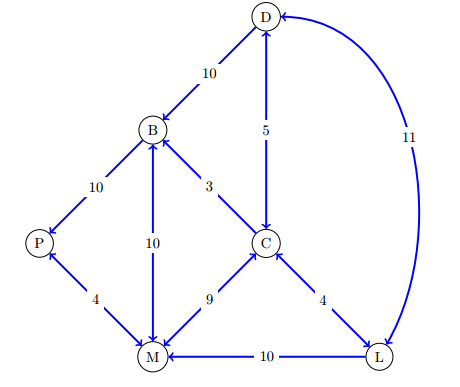
\includegraphics[scale=0.5]{imagenes/grafo.png}
    \end{center}
    \item Desde el vértice $B$ \\
    \begin{center}
        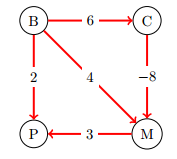
\includegraphics[scale=0.5]{imagenes/grafo2.png}
    \end{center}
\end{itemize}
\newpage
\problem \textbf{Compresión (Huffman)}

Muestre paso a paso la construcción del $trie$ de Huffman para los siguientes Strings y obtenga su compresión respectiva:
\begin{itemize}
    \item AAABCBABBC
    \item ABCBCAAACB
    \item BBBBBBBABC
\end{itemize}

\problem \textbf{Búsqueda en texto (KMP)}

Escriba la función \texttt{prefijoMasLargo} que toma un patrón de largo $m$ y un texto de largo $n$ y retorna el largo máximo de un prefijo del patrón contenido en el texto.\\
La función debe modificar el algoritmo de $Knuth-Morris-Pratt$, por lo que se acepta una complejidad de $\mathcal{O}(n+m)$

\end{problems}



\end{document}


